\documentclass[paper=a4, fontsize=12pt]{scrartcl} % A4 paper and 11pt font size
\usepackage[margin=1in]{geometry}  

\usepackage[T1]{fontenc} % Use 8-bit encoding that has 256 glyphs
\usepackage{fourier} % Use the Adobe Utopia font for the document - comment this line to return to the LaTeX default
\usepackage[english]{babel} % English language/hyphenation
\usepackage{amsmath,amsfonts,amsthm} % Math packages
\usepackage{enumerate}
\usepackage{graphicx}
\usepackage{caption}


\usepackage{sectsty} % Allows customizing section commands
\allsectionsfont{\raggedright \normalfont\scshape} % Make all sections centered, the default font and small caps

\usepackage{fancyhdr} % Custom headers and footers
\pagestyle{fancyplain} % Makes all pages in the document conform to the custom headers and footers
\fancyhead[R]{\emph{Pipe Flow - Chapter 3}} % No page header - if you want one, create it in the same way as the footers below
\fancyfoot[L]{} % Empty left footer
\fancyfoot[C]{} % Empty center footer
\fancyfoot[R]{\thepage} % Page numbering for right footer
\renewcommand{\headrulewidth}{0pt} % Remove header underlines
\renewcommand{\footrulewidth}{0pt} % Remove footer underlines
\setlength{\headheight}{13.6pt} % Customize the height of the header

\numberwithin{equation}{section} % Number equations within sections (i.e. 1.1, 1.2, 2.1, 2.2 instead of 1, 2, 3, 4)
\numberwithin{figure}{section} % Number figures within sections (i.e. 1.1, 1.2, 2.1, 2.2 instead of 1, 2, 3, 4)
\numberwithin{table}{section} % Number tables within sections (i.e. 1.1, 1.2, 2.1, 2.2 instead of 1, 2, 3, 4)

%----------------------------------------------------------------------------------------
%	TITLE SECTION
%----------------------------------------------------------------------------------------

\newcommand{\horrule}[1]{\rule{\linewidth}{#1}} % Create horizontal rule command with 1 argument of height

\author{\vspace{-5ex}}
\date{\vspace{-10ex}}
\title{	
\normalfont \normalsize 
\textsc{Chem-Eng 321: Fluid Mechanics} \\ [10pt] % Your university, school and/or department name(s)
\horrule{0.5pt} \\[0.2cm] % Thin top horizontal rule
\huge Pipe Flow \\ (Denn Chapter 3) \\ % The assignment title
\horrule{2pt} \\[0.2cm] % Thick bottom horizontal rule
}


\begin{document}



\maketitle % Print the title

\thispagestyle{empty}

\section*{Learning Objectives}

\begin{enumerate}
\item Apply dimensional analysis with physical insight and experimental data to find design equations for pipe flow.
\item Describe the laminar and turbulent regimes of fluid pipe flow both qualitatively and quantitatively.
\item  Interpret the numerator and denominator of Reynold's number physically and in relation to laminar and turbulent flow.
\item Derive Poiseuille's law using dimensional analysis and physical insight.
\item Evaluate quantitatively power consumption and cost tradeoffs when designing pipe flow parameters. 
\end{enumerate}

\section*{Dimensional Analysis}

\subsection*{Pipe Flow}

We wish to measure the pressure drop for a fluid through a pipe. The fluid is incompressible and Newtonian. The flow is fully developed. What are potential variables involved?
\\
\\
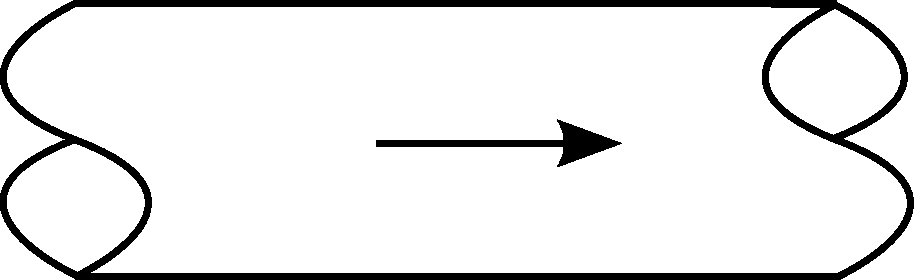
\includegraphics[scale=0.5]{fluidthroughpipe.pdf}

\newpage

How do we figure out how these variables fit into a pipe flow model?

\begin{equation*}
\hspace*{-5cm}  \Delta p=f( 
\end{equation*}

\vspace{5ex}

Traditional Answer:
\vspace{5ex}
\begin{figure}[ht]
\centering
\begin{minipage}[b]{0.3\linewidth}
\includegraphics[scale=0.5]{experiment.pdf}
\end{minipage}
\quad
\begin{minipage}[b]{0.3\linewidth}
\includegraphics[scale=0.5]{experiment.pdf}
\end{minipage}
\quad
\begin{minipage}[b]{0.3\linewidth}
\includegraphics[scale=0.5]{experiment.pdf}
\end{minipage}
\end{figure}
\\
The last experiment doesn't seem particularly feasible. In addition, we'd have to do A LOT of experiments. With six variables where we hold four variables constant for each experiment, we'd have to do \ldots

\vspace{3cm} \subsection*{Introducing Dimensional Analysis}

Dimensional analysis, along with Buckingham $\pi$ theorem, allows us combine variables into dimensionless groups that characterize the process. These dimensionless groups serve as the main parameters describing our model. 

\vspace{2ex}

Buckingham $\pi$ theorem: $G=V-D$ 

\begin{description}
  \item[V] 
  \item[D] 
  \item[G] 
\end{description}

Why?

\newpage

\vspace{10ex} Applying $\pi$ theorem to our above pipe flow example, we have 
\begin{equation*}
G=V-D=6-3=\boxed{3}
\end{equation*}
So if we don't have a model for pipe flow, how do we find our 3 dimensionless groups?

\subsection*{Variables Involved?}

\begin{tabular}{ c || l  }
  Variable & Dimensions (Length, Time, Mass) \\
  $\Delta p$  & $\frac{M}{LT^2}$  \\
   &   \\
   &   \\
   &   \\
   &   \\
   &   \\
   &   \\
   &   \\
   &   \\
   &   \\
   &   \\
   &   \\
   &   \\
   &   \\
   &   \\
\end{tabular}


\vspace{5ex} Messing around:

\vspace{15ex}

We need something with $\Delta p$

\newpage

Lots of groups; many more than 3! What's going on?

\vspace{15ex}

Which 3 should we pick?
\begin{enumerate}
  \item
  \item \vspace{10ex} We wish to see how $\Delta p$ depends on the other variables, so let's select only \underline{one} group with that.
  \item \vspace{20ex}
\end{enumerate}


\vspace{20ex} Dimensional Analysis tells us that we can go from
\vspace{5ex} \begin{equation*}
\hspace*{-7cm}  \Delta p=f( 
\end{equation*}
\vspace{2ex} \begin{equation*}
\hspace*{-5cm}  \Downarrow
\end{equation*}


\newpage

\subsection*{Using physical insight}
We found appropriate dimensionless groups through dimensional analysis, now using physical insight, we can simplify further. Consider two sections of pipes.

\begin{figure}[ht]
\centering
\begin{minipage}[b]{0.40\linewidth}
\includegraphics[scale=0.3]{fluidthroughpipe2.pdf}
\end{minipage}
\quad
\begin{minipage}[b]{0.55\linewidth}
\includegraphics[scale=0.3]{fluidthroughpipe3.pdf}
\end{minipage}
\end{figure}

\vspace{10ex} This insight allows us to characterize our model further

\vspace{10ex} And now we can define the \underline{Fanning friction factor} (f) and \underline{Reynold's number} (Re).
\vspace{2ex} \begin{equation*}
\hspace*{-5cm}  \text{f}=
\end{equation*}
\vspace{2ex} \begin{equation*}
\hspace*{-5cm} \text{Re}=
\end{equation*}

\begin{equation*}
\boxed{\text{f}=f(\text{Re})}
\end{equation*}

\subsection*{Experiments}
We were successfully able to apply dimensional analysis and physical insight to relate two parameters and perform only one experiment!

\includegraphics[scale=0.6]{experiment2.pdf}

\newpage

Data
\begin{itemize}
  \item Different
  \item Different
  \item Different
  \item Different
\end{itemize}
"Dynamic Similarity" (DVD pp 534-540; 568-601)

\subsection*{Reynolds Experiment}
(DVD pp 730-733)

\begin{figure}[ht]
\centering
\begin{minipage}[b]{0.45\linewidth}
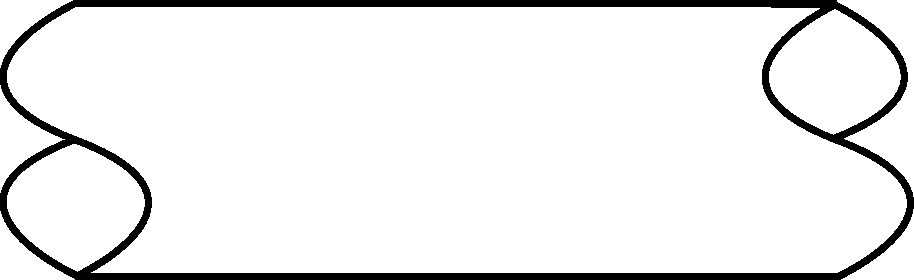
\includegraphics[scale=0.4]{fluidthroughpipe4.pdf}
\caption*{Re < 2100}
\end{minipage}
\quad
\begin{minipage}[b]{0.45\linewidth}
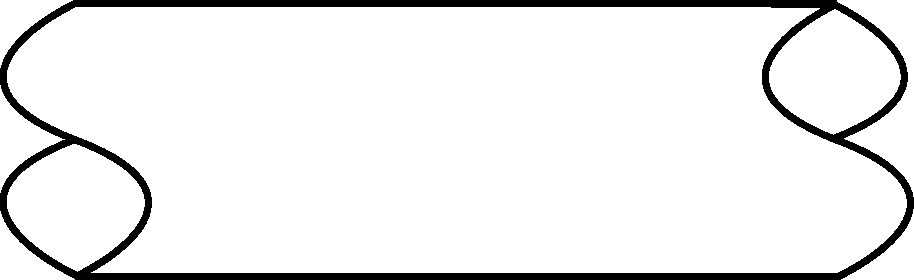
\includegraphics[scale=0.4]{fluidthroughpipe4.pdf}
\caption*{Re > 2100}
\end{minipage}
\end{figure}
\hspace*{2cm} \begin{tabular*}{11cm}{c @{\extracolsep{\fill}} c}
\underline{Laminar Flow} & \underline{Turbulent Flow} \\
$v_z=v_z(r)$ & $v_z=v_z(r,\theta,z,t)$ \\
$v_r=0$ & $v_r=v_r(r,\theta,z,t)$ \\
$v_\theta=0$ & $v_\theta=v_\theta(r,\theta,z,t)$ \\
\end{tabular*}
\newpage
\subsection*{Another Dimensional Analysis Example}

Liquid is slowly dripping out of a faucet of diameter $D$ under the influence of gravity $g$. The liquid has density $\rho$ and surface tension $\sigma$ (dimensions force/length). Using dimensional analysis, determine how fluid mass $M$ will relate to the other variables in the problem. 

\newpage

\section*{Pipe Flow Data Correlations}

\subsection*{Re < 2100}

Laminar flow $\rightarrow$ 

\vspace{1cm} \begin{equation*}
\hspace*{-8cm}  Q=  \hspace*{4cm}  \Rightarrow v=\frac{Q}{A} = 
\end{equation*}

\vspace{1cm} Now rearrange to

\vspace{1cm} Multiply both by...

\vspace{1cm} \begin{equation*}
\hspace*{-2cm}  \hspace*{4cm} = \hspace*{4cm}  
\end{equation*}

\vspace{1cm} \begin{equation*}
\hspace*{-2cm}  \hspace*{-2cm}  \text{f}  = \hspace*{4cm}  
\end{equation*}

\vspace{0.5cm}  \subsection*{Re > 2100}
Turbulent flow $\rightarrow$ 

\vspace{0.25cm} \subsubsection*{ Empirical Equations }


\vspace{0.25cm}  Blasius Equation
\begin{equation*}
\hspace*{-8cm}  \text{f}=
\end{equation*}
\vspace{0.25cm}  von Karman-Nikuradse correlation
\begin{equation*}
\hspace*{-8cm} \frac{1}{ \sqrt{\text{f}}}=
\end{equation*}


\vspace{1.5cm}  \subsubsection*{2100 < Re <4000}




\newpage 

\subsubsection*{Chart}

\includegraphics[scale=0.9]{Figure3-1.png}

\vspace{-1cm}  \subsection*{Example Problem}

Water is pumped through 50m of a smooth pipe with an inside diameter of 5cm at a volumetric flow rate of 4 liters/second. What is the pressure drop? 



\newpage

\section*{Physical Interpretation of Reynold's Number}

Reynold's number can be thought of the ratio between \underline{inertial} forces and \underline{viscous} forces. (DVD pp. 496-508).
\begin{equation*}
\text{Re}=\frac{\text{Inertial Forces}}{\text{Viscous Forces}}
\end{equation*}

\subsection*{Inertial forces}
Inertia is what must be overcome to change speed/direction of a fluid. Consider a blob of fluid impinging on a wall with mass $M$, moving at velocity $V$, with a distance $\Delta l$ to the wall. 
\vspace{1cm} \begin{equation*}
\hspace*{-1cm}  \text{Inertial Force}=F_{I}=
\end{equation*}

\vspace{5 cm} \subsection*{Viscous Forces}
Viscous forces are associated with deformation of a fluid. Consider a blog of fluid moving parallel to the wall.

\vspace{1.5cm} \hspace*{6cm}  Shear rate $ \Gamma_{s} \approx $

\vspace{1.5cm} \hspace*{6cm}  Shear stress $ \tau_{s} \approx $

\vspace{1.5cm} \hspace*{6cm}  Viscous Force $ F_{V} \approx $

\newpage
\subsection*{Ratio}
\begin{equation*}
\hspace*{-8cm} \frac{F_{I}}{F_{V}}=
\end{equation*}

\vspace{5 cm} \subsection*{Revisiting Dimensional Analysis for Laminar Pipe Flow}
Streamlines are straight, there is constant velocity (no acceleration), so therefore \dots

\newpage
~
\vspace{2cm} \begin{equation*}
\hspace*{-8cm}  Q \propto
\end{equation*}


\vspace{3cm} We obtained a mathematical form of Poiseuile's law without a detailed solution using only dimensional analysis and physical insight!

\subsection*{Corollary}
 \begin{equation*}
\hspace*{-8cm}  \text{f}= 
\end{equation*}

\vspace{2cm} 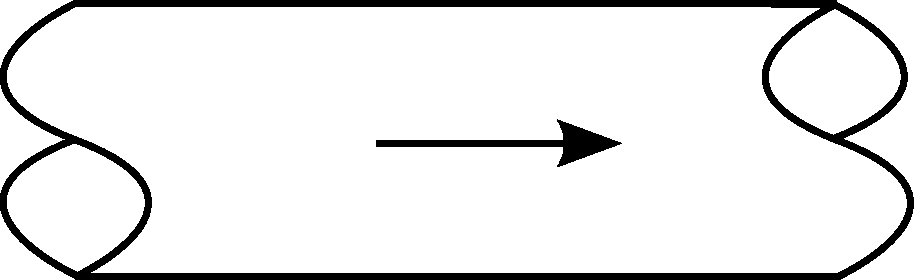
\includegraphics[scale=0.4]{fluidthroughpipe.pdf}

\newpage

\section*{Power Requirement for Pumping}
 \begin{equation*}
\vspace{1cm} \hspace*{-10cm}  \text{Power}= 
\end{equation*}

For Pipe flow: 

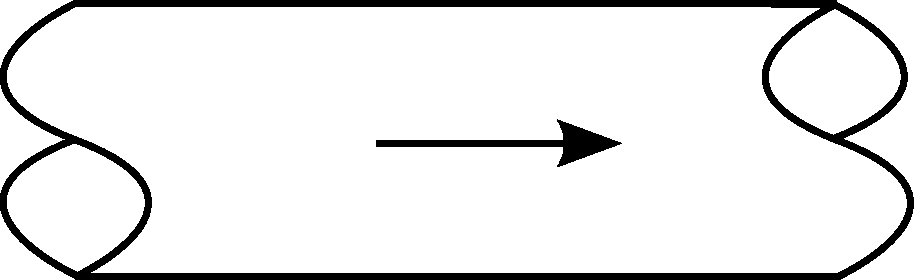
\includegraphics[scale=0.4]{fluidthroughpipe.pdf}
~
 \begin{equation*}
\vspace{1cm} \hspace*{-10cm}  \text{Work}= 
\end{equation*}

\vspace{1cm}  Over time $\Delta t$, the fluid moves distance $\Delta l$

 \begin{equation*}
\vspace{1cm} \hspace*{-10cm}  \text{Power}= 
\end{equation*}

 \begin{equation*}
\vspace{1cm} \hspace*{-10cm}  \text{Power}= 
\end{equation*}

\section*{Optimal Pipe Diameter}

We want to pump fluid distance $L$ with volumetric flow rate $Q$. What pipe diameter do we choose? How do we choose?


 \vspace{2cm}  \begin{equation*}
\hspace*{-6cm}  \text{Total Cost}= \text{Operating Cost} + \text{Capital Costs}
\end{equation*}

\subsection*{Capital Costs}

\vspace{3cm}  \begin{equation*}
\hspace*{-10cm}  \text{Capital Costs}= 
\end{equation*}

\subsection*{Operating Costs}

\vspace{10cm}  \begin{equation*}
\hspace*{-10cm}  \text{Operating Costs}= 
\end{equation*}

\subsection*{Total Costs}

\begin{equation*}
\hspace*{-9cm}  \text{Total Cost}= 
\end{equation*}

\vspace{3cm} \includegraphics[scale=0.6]{costvsd.pdf}

\newpage
\subsection*{Solving for optimal diameter}

\vspace{4cm}  \section*{Rough Pipe}

\vspace{1cm} \includegraphics[scale=0.8]{surface.pdf}

 \vspace{1cm}   Dimensional Analysis... add a new variable

\begin{equation*}
\hspace*{-6cm}  \text{f}= f(
\end{equation*}

 \vspace{1cm}  Experiments, Nikuradse (glue sand to pipes)

 \vspace{1cm}  \includegraphics[scale=0.6]{experiment2.pdf}
 
\vspace{1cm}  Estimating f in rough pipes: Colebrook formula

\begin{equation*}
\hspace*{-6cm}  \frac{1}{\sqrt{\text{f}}}= 
\end{equation*}

\vspace{1cm}   \begin{enumerate}
\item Calculate
\item Calculate
\item  Use the formula or chart to determine f
\end{enumerate}

\subsection*{Commercial Pipes}




\vspace{3cm}  \section*{Non-circular Cross Sections}
For turbulent flow...

\vspace{1cm}   \begin{enumerate}
\item Define the hydraulic diameter: $D_H=$
\vspace{6cm} \item Use $D_H$ in place of $D$ in calculating 
\vspace{1cm} \item  Use correlations for circular tubes
\end{enumerate}

\newpage
\subsection*{Example Problem}
Water is pumped through 20 m of a channel with a square cross section (see below) with B=50 mm. The channel is made from commercial steel with a surface roughness of $k=0.05$ mm. What will be pressure drop assuming the average fluid velocity is 4 m/s. Assume $\rho=1000 \frac{\text{kg}}{\text{m}^3}$ and $\eta=0.001$ Pa s

\vspace{1cm}  \includegraphics[scale=0.8]{hiptobesquare.pdf}

\newpage
\section*{Chapter Summary}
Aim: To develop a fluid model for pipe flow as a function of known, involved parameters without a detailed flow solution (macroscopically).

\vspace{1cm}  Challenge:

\vspace{1cm}  Solution: Apply Dimensional Analysis and

\vspace{1cm}  Additionally, dimensional analysis allows us to 
\begin{itemize}
  \item Simplify the our model by reducing number of parameters (and thus experiments)
  \item 
  \item
\end{itemize}

For simple pipe flow, we found two dimensionless groups to characterize flow through a pipe, Reynold's Number (Re) and Fanning Friction factor (f).

\vspace{1cm}  Reynold's Number reveals the following about fluid flow:
\begin{itemize}
  \item The balance of viscous and inertial forces (laminar vs turbulent regime).
  \item The correlation/equation to be used with friction factor. 
\end{itemize}

From experiments and derivations we can relate friction factor to Reynold's number. 

Using pipe flow models we can

\begin{itemize}
  \item Calculate the power requirement
  \item Find optimal sizing for our process
  \item Account for 
  \item Account for 
\end{itemize}

\newpage

\section*{Appendix A}

 \includegraphics[scale=.90]{StandardPipeSizes.pdf}
 
 \newpage

\section*{Appendix B}

 \includegraphics[scale=0.9]{Figure3-1.png}
 
  \includegraphics[scale=0.9]{MoodyChart.png}

\end{document}

